\chapter{Analysis Results}
\label{ch:Results}

The analysis presented in this dissertation was designed to make several measurements. As this dissertation was written alongside the first \nova~NC analysis, one primary goal of the analysis was to demonstrate the successful ability of \nova~to identify NC events and measure the ratio of observed to predicted NC events in a 3 flavor hypothesis, $R_{NC}$.
\beq
R_{NC} \equiv \frac{ N_{Obs} - N_{Pred}^{Bkg} }{ N_{Pred}^{NC} }
\label{eq:R}
\eeq

\n The other (arguably more important) goal was to start contributing to the global data on the sterile mixing parameters by extracting measurements on the mixing angles $\theta_{24}$, $\theta_{34}$ and matrix elements $\Usqxy{\mu}{4}$ and $\Usqxy{\tau}{4}$.

Results in this chapter were collected between February 2014 and May 2016. For the FD, this corresponds to \pot{6.69}, or $6.05 \times 10^{20}$ full detector equivalent POT. For the ND, \pot{3.71} was collected.

The first section in this chapter describes the fitting methods used to make the mixing angle and matrix element measurements. Before presenting the results, the next two sections discuss preliminary tests to demonstrate satisfactory performance of the analysis. The final section in this chapter presents the ultimate results.

\section{Fitting Method}

It was decided to make rate only measurements for the first \nova~NC disappearance analysis. Thus, even though the extrapolation and prediction were performed in $250\unit{MeV}$ bins of calorimetric energy, only the integrated event totals were input to the fitting framework.

Fitting was performed allowing some parameters to float, some held to best fit values, and others set to 0 due to insensitivity. As mentioned above, a major analysis goal was to measure $\theta_{24}$ and $\theta_{34}$, so these angles were allowed to float between $0^\circ$ and $45^\circ$. Values outside of this range are either equivalent to this range through redefinition of the angles, or already highly disfavored through previous experiments and in a region difficult for fitting due to many local minima. $\theta_{23}$ was allowed to float with a Gaussian constraint with mean $45.8^\circ$ and standard deviation $3.2^\circ$, the best fit measurement by T2K \cite{ref:T2K2015}. All of the remaining parameters were held fixed to the values listed in table \ref{tab:FitFix}.
\begin{table}[htb]
  \begin{center}
    \caption[Fixed Parameters and Values for Fitting]{The parameters held fixed and the values they were set at for fitting.}
    \label{tab:FitFix}
    \begin{tabular}{c c}
      \hline\hline
      Parameter & Value \\
      \hline
      $\dmxy{1}{2}$ & $7.53 \times \left[10^{-5}\evsq\right]$ \\
      $\dmxy{2}{3}$ & $2.37 \times \left[10^{-3}\evsq\right]$ \\
      $\sin^2 2\theta_{12}$ & $0.846$ \\
      $\sin^2 2\theta_{13}$ & $0.085$ \\
      $\theta_{14}$ & $0$ \\
      $\delta_{13}$ & $0$ \\
      $\delta_{24}$ & $0$ \\
      $\delta_{14}$ & $0$ \\
      \hline
    \end{tabular}
  \end{center}
\end{table}

The best fit values were found by calculating the minimum $\chi^2$ value and allowing individual systematics to float with a penalty,
\beq
\chi^2 = 2 \left( N_{Pred} - N_{Obs} + N_{Obs} \ln \frac{N_{Obs}}{N_{Pred}} \right) + \left( \frac{ \theta_{23} - \mu_{23} }{ \sigma_{23} } \right)^2 + \sum_{i=1}^{N} \left( \frac{ \sigma_i^{BF} }{\sigma_i} \right)^2,
\label{eq:Chisq}
\eeq
\n where $\mu_{23}$ and $\sigma_{23}$ are the mean and standard deviation used in the Gaussian constraint on the value of $\theta_{23}$, $\sigma_i^{BF}$ is the number of standard deviations the $i$th systematic error is shifted in the best fit, and $\sigma_i$ is one standard deviation for the $i$th systematic error. Equation \ref{eq:Chisq} is the standard formula for calculating $\chi^2$ with penalty terms, where the first term is the basic value for $\chi^2$, and the second and third terms add a unit for each shift of $\theta_{23}$ and the systematic errors by their respective variances. For one and two dimensional $\chi^2$ surfaces, the remaining angles not shown were profiled.

\section{ND Data/MC Comparisons}

Before diving head first into the FD data, the first necessary analysis benchmark was ND data/MC comparisons. Fig~\ref{fig:NDDataMCECal} shows the event energy distributions and fig.s \ref{fig:NDDataMCFidCont}, \ref{fig:NDDataMCNCSel}, and \ref{fig:NDDataMCCosRej} show the distributions for all of the variables used for selection discussed in chapter \ref{ch:Selection}.
\begin{figure}[htbp]
  \centering
  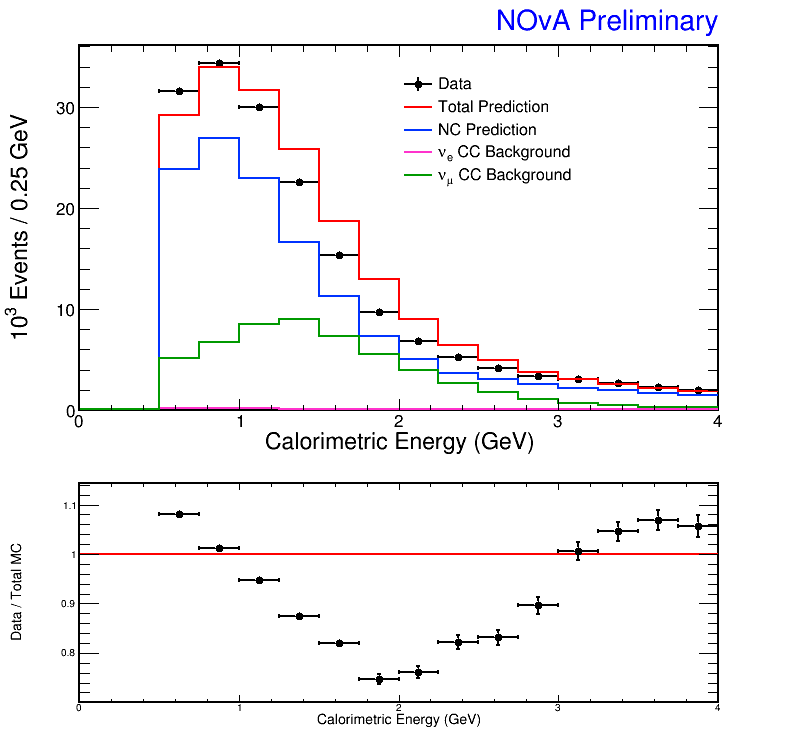
\includegraphics[width=1\textwidth]{figures/NDDataMC/ECalNusNDRat.png}
  \caption[ND Data/MC Comparison: Energy Distribution]{ND data/MC comparison of the calorimetric energy.}
  \label{fig:NDDataMCECal}
\end{figure}

\begin{figure}[htbp]
  \centering
  \begin{tabular}{c c}
    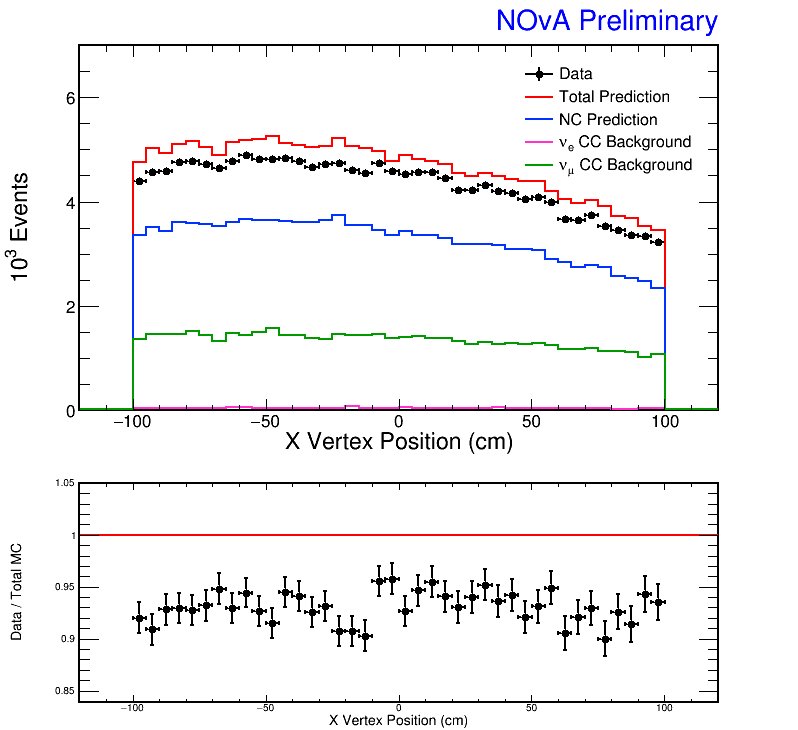
\includegraphics[width=.47\textwidth]{figures/NDDataMC/VtxXNusNDRat.png} &
    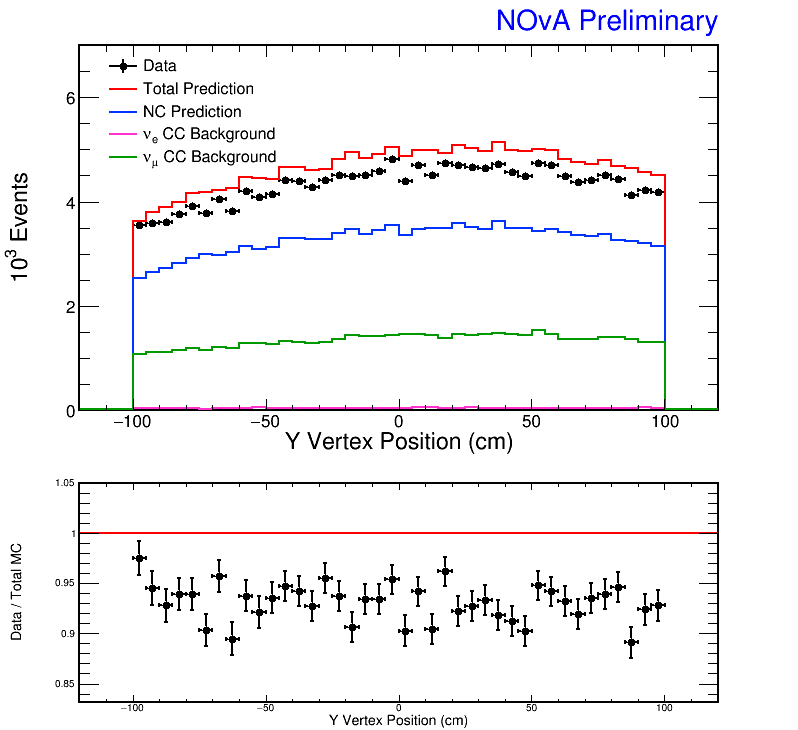
\includegraphics[width=.47\textwidth]{figures/NDDataMC/VtxYNusNDRat.png} \\
    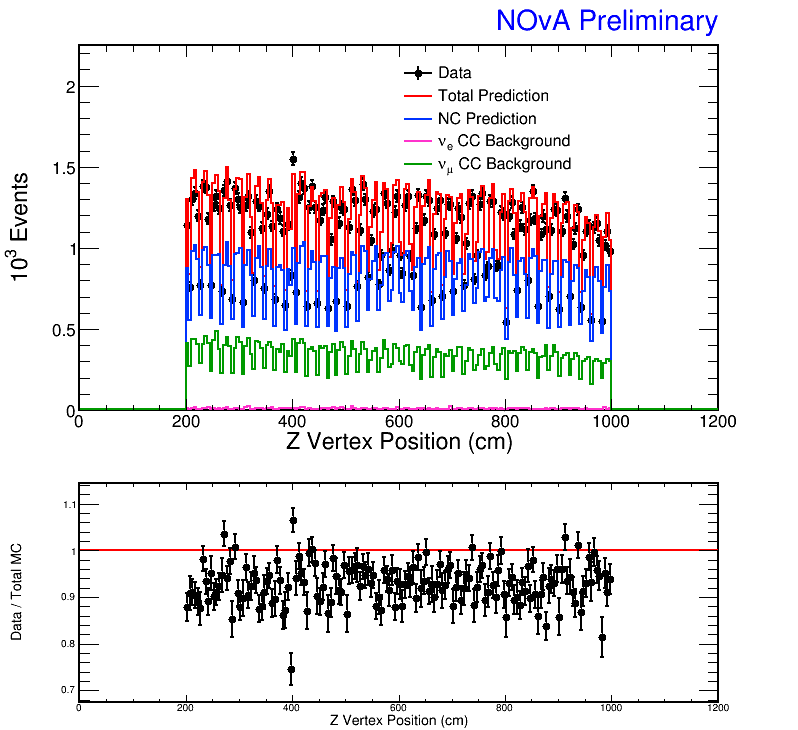
\includegraphics[width=.47\textwidth]{figures/NDDataMC/VtxZNusNDRat.png} &
    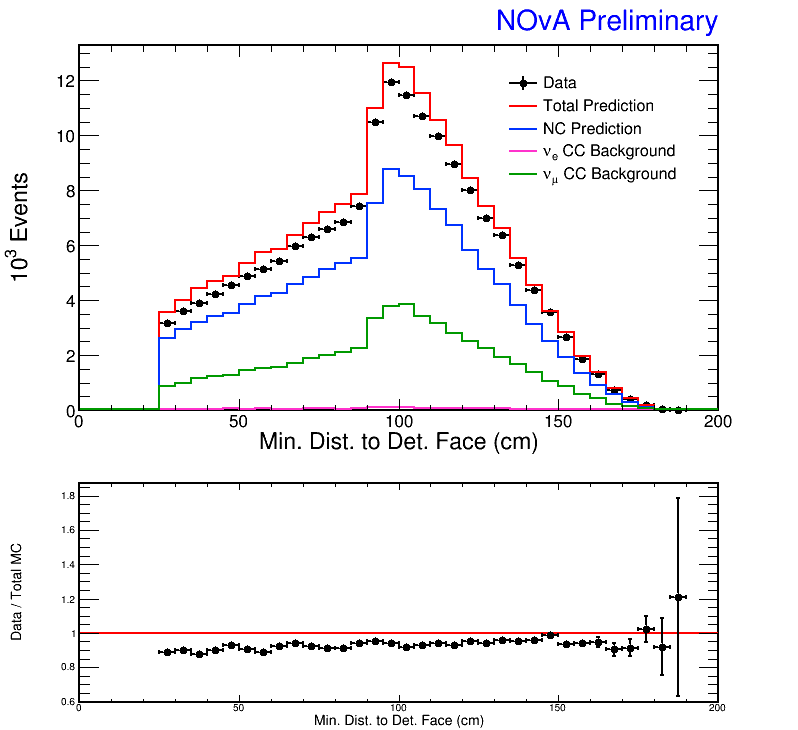
\includegraphics[width=.47\textwidth]{figures/NDDataMC/ContNusNDRat.png} \\
  \end{tabular}
  \caption[ND Data/MC Comparison: Fiducial and Containment Variable Distributions]{ND data/MC comparison of the reconstructed vertex position and containment distributions.}
  \label{fig:NDDataMCFidCont}
\end{figure}

\begin{figure}[p]
  \centering
  \begin{tabular}{c c}
    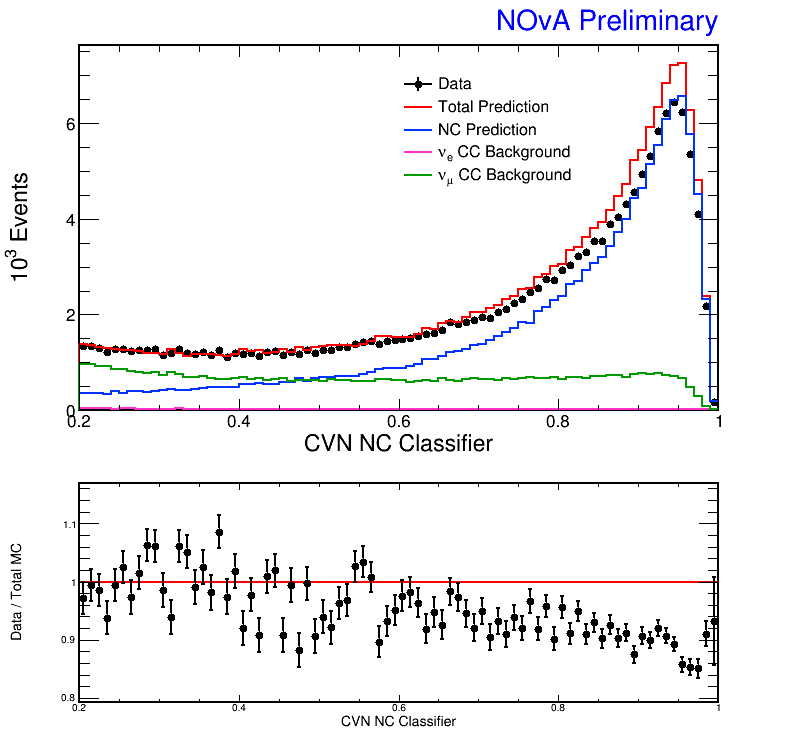
\includegraphics[width=.47\textwidth]{figures/NDDataMC/CVNNusNDRat.png} &
    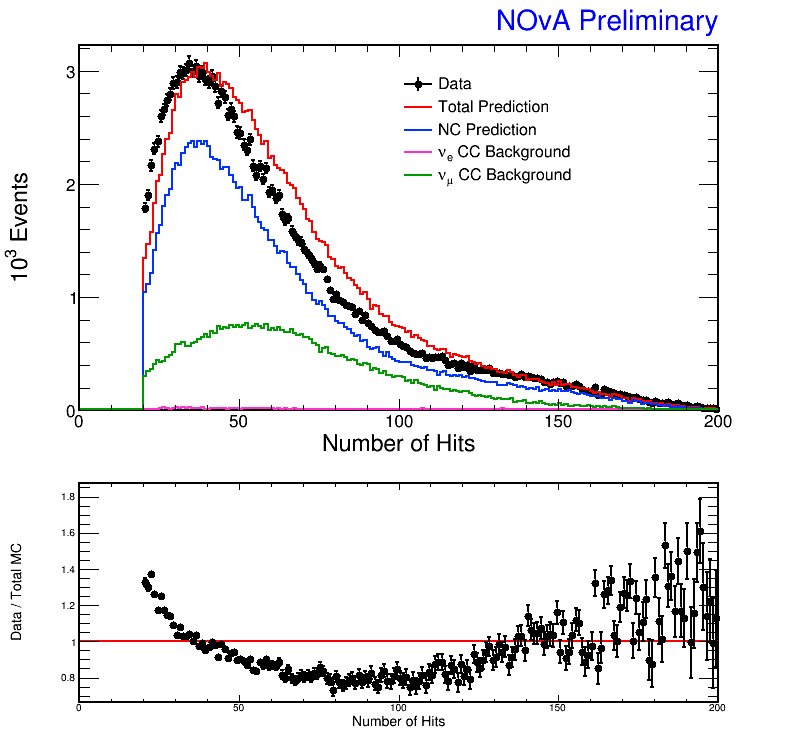
\includegraphics[width=.47\textwidth]{figures/NDDataMC/NHitNusNDRat.png} \\
  \end{tabular}
  \caption[ND Data/MC Comparison: NC Selection Variable Distributions]{ND data/MC comparison of the CVN and number of hits distributions.}
  \label{fig:NDDataMCNCSel}
\end{figure}

\begin{figure}[p]
  \centering
  \begin{tabular}{c c}
    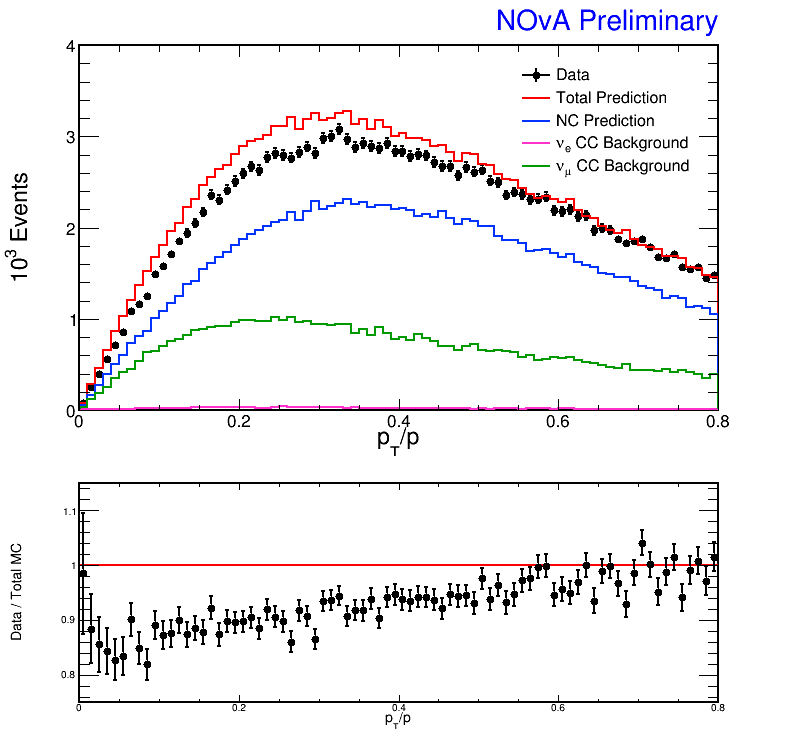
\includegraphics[width=.47\textwidth]{figures/NDDataMC/PTPNusNDRat.png} &
    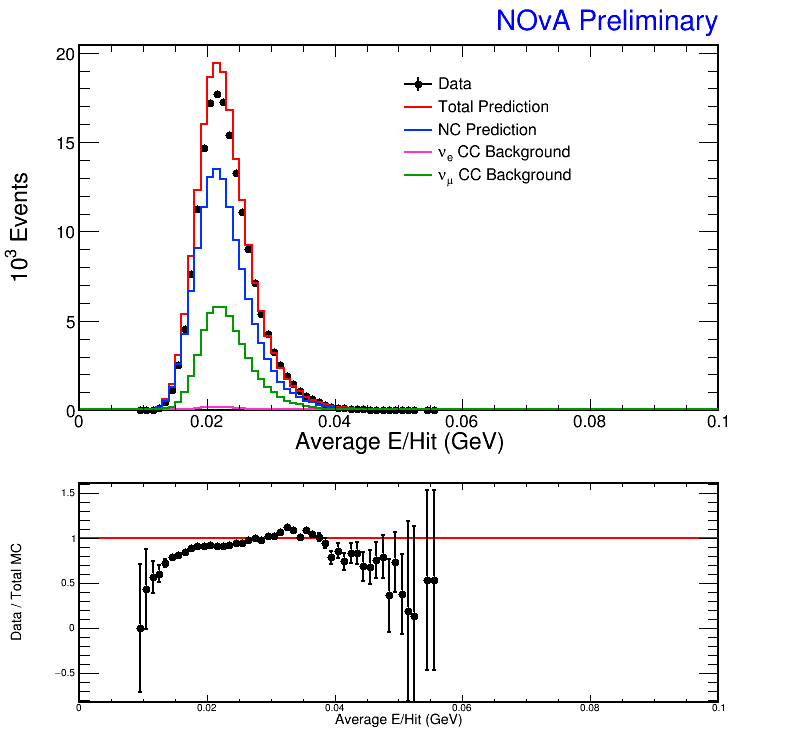
\includegraphics[width=.47\textwidth]{figures/NDDataMC/EpHNusNDRat.png} \\
  \end{tabular}
  \caption[ND Data/MC Comparison: Cosmic Rejection Variable Distribution]{ND data/MC comparison of particle transverse momentum and energy per hit distributions.}
  \label{fig:NDDataMCCosRej}
\end{figure}

\n While most of the distributions differ by at most a small normalization, a few have an apparent shift, notably the energy and number of hits distributions. These particular discrepancies were actually expected due to a known mismodeling of NC interactions.

Very recently there was experimental evidence for a new `mode' of interaction. A systematic scale for this event type was added to and evaluated with the GENIE systematics discussed in section \ref{sec:SystGENIE}. The inclusion of these effects drastically improved the data/MC agreement for the \nova~CC analyses. Unfortunately, while the experimental data was available allowing for study of these effects on CC events, the data for NC events is largely nonexistent. Consequently the \nova~simulation does not include these effects for NC events despite widespread belief that similar effects should be seen. This would largely explain the data/MC differences seen in the energy and number of hits distributions.

Two sanity checks were performed to ensure that the data/MC difference would not negatively impact the analysis. First, the ND data/MC energy distribution was shown with a full systematic error band to show the difference is covered by systematics. This was shown in figure \ref{fig:NDSystBand}. Secondly, the effect of shifting either the data or MC in relation to the other on the predicted event rate and 1D angle sensitivities was studied. This was done by shifting the data up or the MC down by the ratio of the means of the energy distributions for MC and data, $1.39\unit{GeV} / 1.33\unit{GeV} \approx 4.5\%$ and also for a much larger shift of $10\%$. The event counts are shown in table \ref{tab:FDShift} and the angle sensitivities are shown in figure \ref{fig:1D2434Shift}. Due to the nature of a counting experiment, since the overall event rates are essentially unchanged, the effect of these rather large shifts is negligible. As a result, it was decided to take the data and MC as is and push for model improvements for future analyses.
\begin{table}[htb]
  \begin{center}
    \caption[FD Event Rates for Shifted Energy Spectra]{The number of predicted events at the FD after applying an energy shift to data or MC.}
    \label{tab:FDShift}
    \begin{tabular}{c c c c c c c}
      \hline\hline
      Shift & All & NC & $\numu$ CC & $\nue$ CC & Cosmic & FOM \\
      \hline
      Nominal & 83.5 & 60.6 & 4.6 & 3.6 & 14.3 & 6.633 \\
      Data $4.5 \%$ Up & 84.6 & 61.0 & 4.7 & 3.7 & 14.9 & 6.634 \\
      Data $10 \%$ Up & 86.2 & 61.4 & 4.9 & 3.7 & 15.8 & 6.612 \\
      MC $4.5 \%$ Down & 85.1 & 61.8 & 4.8 & 3.7 & 14.3 & 6.702 \\
      MC $10 \%$ Down & 87.2 & 63.4 & 5.2 & 3.8 & 14.3 & 6.792 \\
      \hline
    \end{tabular}
  \end{center}
\end{table}

\begin{figure}[htb]
  \centering
  \begin{tabular}{c c}
    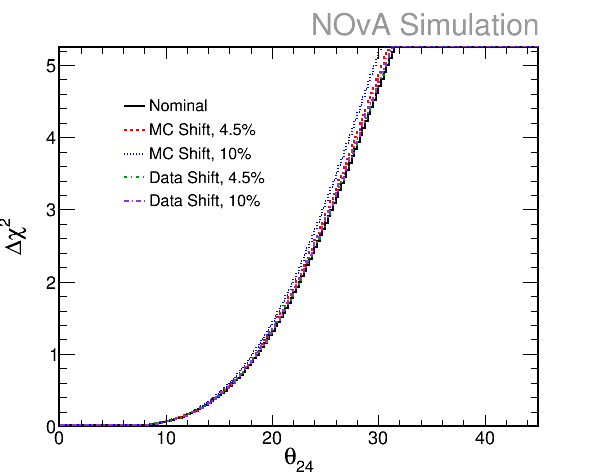
\includegraphics[width=.47\textwidth]{figures/EShift24.png} &
    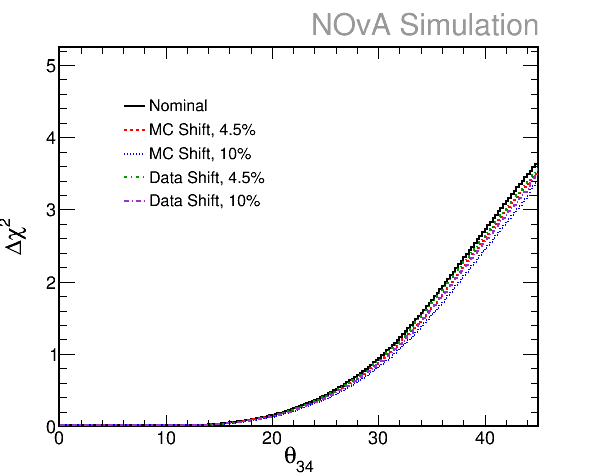
\includegraphics[width=.47\textwidth]{figures/EShift34.png} \\
  \end{tabular}
  \caption[Angle Sensitivities for Shifted Energy Spectra]{Angle sensitivities after applying an energy shift to either MC or data. Left: $\theta_{24}$, Right: $\theta_{34}$. The fits are statistics only and do not include any systematic errors.}
  \label{fig:1D2434Shift}
\end{figure}

\section{Sideband Studies}

Three different sidebands were studied to test the performance of the analysis, a high energy sideband, a low CVN sideband, and mid cosmic BDT sideband. The predicted and observed event rates for each sideband are shown in table \ref{tab:Sideband}.
\begin{table}[htbp]
  \begin{center}
    \caption[Sideband Event Rates]{The observed and predicted events at the FD for each sideband.}
    \label{tab:Sideband}
    \begin{tabular}{c c c c c c c}
      \hline\hline
      Sideband & Data & Total MC & NC & $\numu$ CC & $\nue$ CC & Cosmic \\
      \hline
      High Energy & 15 & 8.2 & 6.5 & 0.8 & 0.5 & 0.1 \\
      Low CVN & 35 & 32.7 & 3.7 & 5.5 & 19.3 & 4.0 \\
      Mid BDT & 17 & 14.5 & 6.0 & 0.5 & 0.4 & 7.5 \\
      \hline
    \end{tabular}
  \end{center}
\end{table}

The high energy sideband applied the standard selection and considered events between $4$ and $6\unit{GeV}$, a region chosen due to its high purity of NC events. The predicted and observed event distributions are shown in figure \ref{fig:SidebandHighE}, $8.2$ events were predicted and $15 \pm 4$ were observed in data. While the observed rate is slightly high, the low statistics means that the observation is within $2\sigma$ of the prediction. Furthermore, the discrepancy is largely driven by a single bin rather than a systematic offset. This result was thus interpreted as validation for the general analysis procedure.
\begin{figure}[htbp]
  \centering
  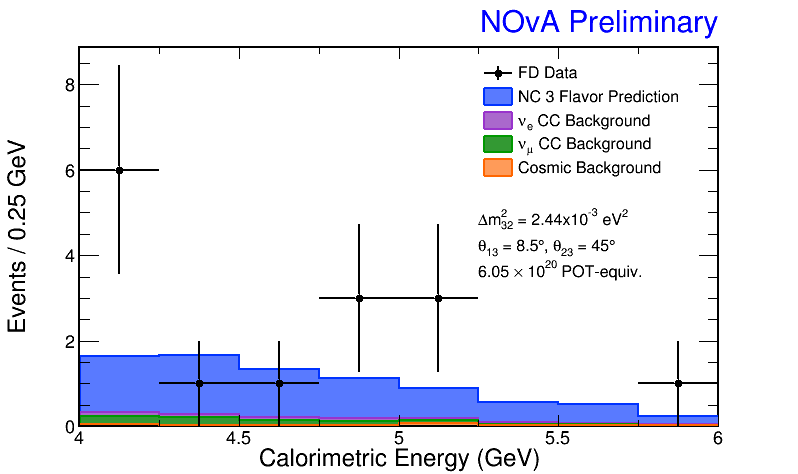
\includegraphics[width=1\textwidth]{figures/Ana01Results/FDHighECalEDataMCStack.png}
  \caption[High Energy Sideband]{The observed and predicted FD event rates for the high energy sideband.}
  \label{fig:SidebandHighE}
\end{figure}

The low CVN sideband considered events that fail the CVN cut, or those with a CVN NC score below $0.2$. This region was used as validation for the CVN selector. The predicted and observed event distributions are shown in figure \ref{fig:SidebandLowCVN}, $32.7$ events were predicted and $35 \pm 6$ were observed in data. The overall agreement in both shape and rate for this sideband provided great confidence in the performance of CVN.
\begin{figure}[htbp]
  \centering
  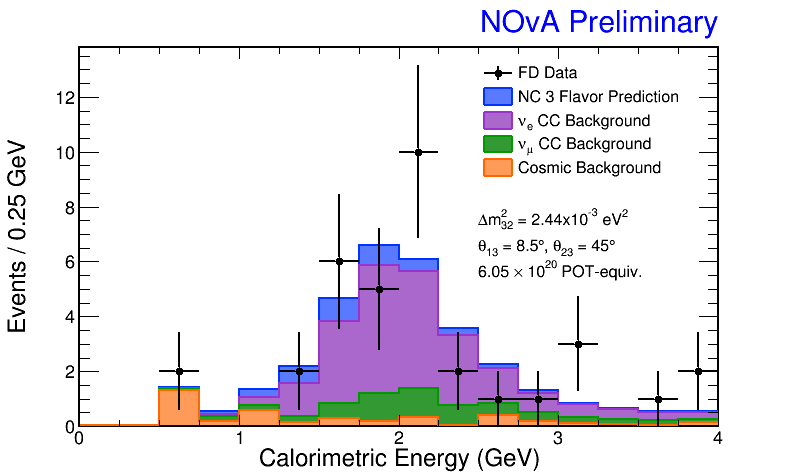
\includegraphics[width=1\textwidth]{figures/Ana01Results/FDLowCVNCalEDataMCStack.png}
  \caption[Low CVN Sideband]{The observed and predicted FD event rates for the low CVN sideband.}
  \label{fig:SidebandLowCVN}
\end{figure}

The mid cosmic BDT sideband considers events with a BDT score between $0.42$ and $0.5$, a region which fails the standard selection cuts but still has NC events. The predicted and observed event distributions are shown in figure \ref{fig:SidebandMidBDT}, $14.5$ events were predicted and $17 \pm 4$ were observed in data. This sideband also showed excellent agreement in both shape and rate, providing further validation for the general analysis procedure, and specifically for the main cosmic rejection variable.
\begin{figure}[htbp]
  \centering
  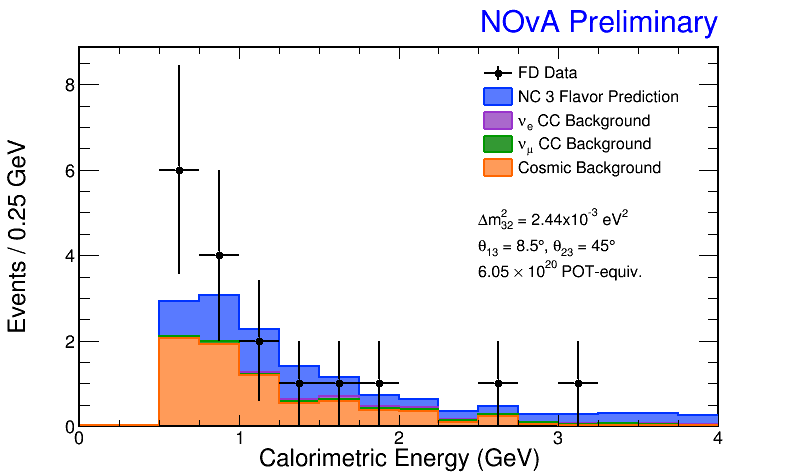
\includegraphics[width=1\textwidth]{figures/Ana01Results/FDMidBDTCalEDataMCStack.png}
  \caption[Mid Cosmic BDT Sideband]{The observed and predicted FD event rates for the mid cosmic BDT sideband.}
  \label{fig:SidebandMidBDT}
\end{figure}

\section{Results}

This analysis predicted that there would be $83.8 \pm a.b \mbox{(stat.)} ^{+c.d}_{-e.f} \mbox{(syst.)}$ NC-like events selected in the FD data. $95 \pm 9.7$ were observed, corresponding to a measurement of $R_{NC} = 1.186 \pm 0.161 \mbox{(stat.)} ^{+0.081}_{-0.129} \mbox{(syst.)}$ If active neutrinos mixed with sterile neutrinos, the number of observed events would be depleted, causing $R_{NC}$ to be less than one. Thus, the measurement of $R_{NC}$ is consistent with the no sterile mixing hypothesis.

The energy distribution of the predicted and observed events is shown in figure \ref{fig:FDDataMCECal}. The $\chi^2$ of this distribution is $23.31$ for $14$ bins, or $1.665$/bin. To better assess the understanding of the observed data, data/MC comparisons distributions were studied for many of the variables used for selection, including regions cut for the analysis. These can be seen in fig.s \ref{fig:FDDataMCFidCont}, \ref{fig:FDDataMCNCSel}, and \ref{fig:FDDataMCCosRej}.
\begin{figure}[htbp]
  \centering
  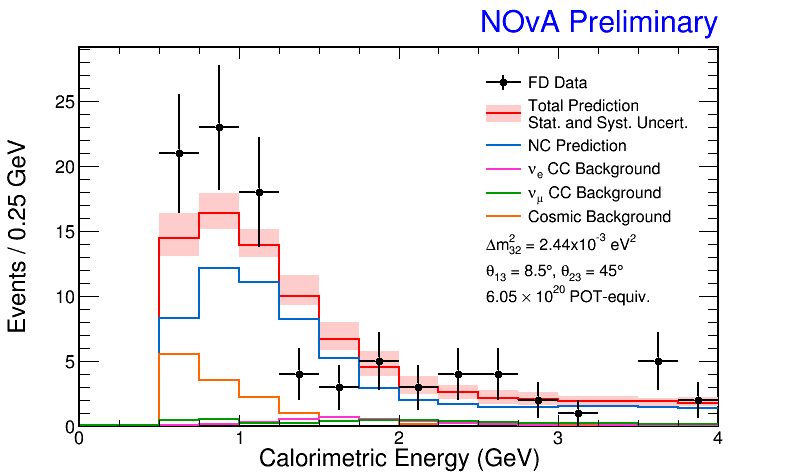
\includegraphics[width=1\textwidth]{figures/FDDataMC/cCalEFDAllStSy.png}
  \caption[FD Data and MC Energy Distribution]{Calorimetric energy distribution of events predicted and observed in the FD.}
  \label{fig:FDDataMCECal}
\end{figure}

\begin{figure}[htbp]
  \centering
  \begin{tabular}{c c}
    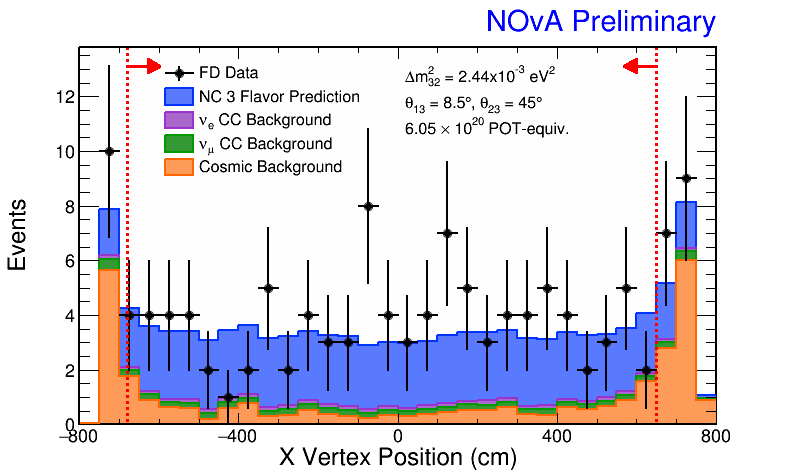
\includegraphics[width=.47\textwidth]{figures/FDDataMC/FDVtxXStack.png} &
    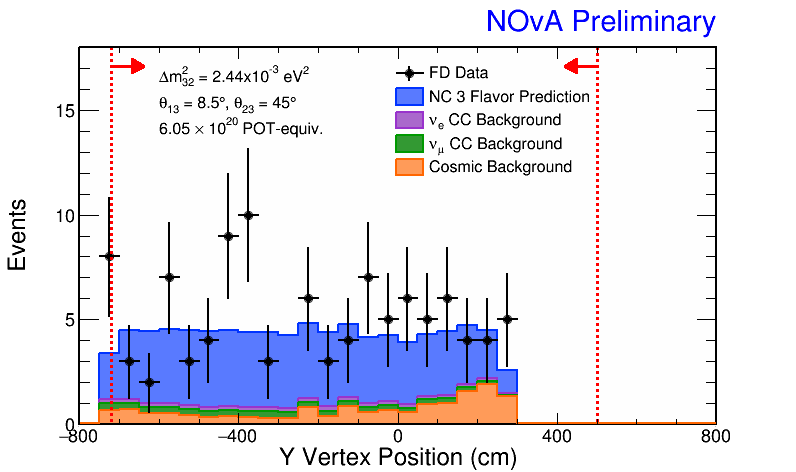
\includegraphics[width=.47\textwidth]{figures/FDDataMC/FDVtxYStack.png} \\
    \multicolumn{2}{c}{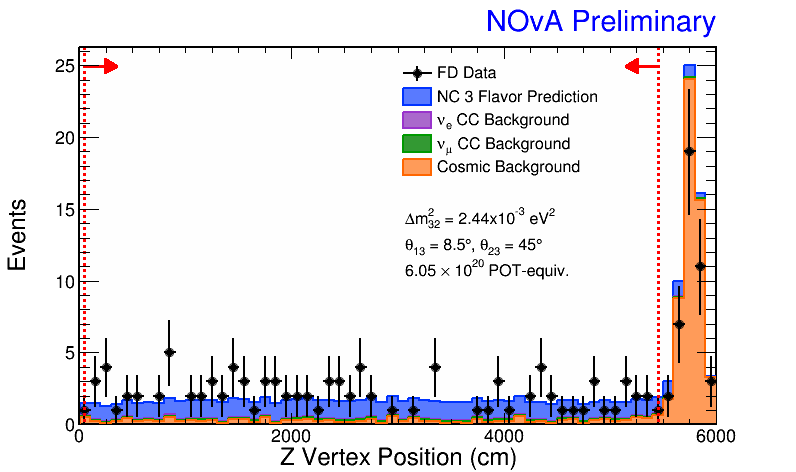
\includegraphics[width=.47\textwidth]{figures/FDDataMC/FDVtxZStack.png}} \\
  \end{tabular}
  \caption[FD Data/MC Comparison: Fiducial Variable Distributions]{FD data/MC comparison of the reconstructed vertex position distributions. The dashed lines and arrows indicate the regions kept for the analysis.}
  \label{fig:FDDataMCFidCont}
\end{figure}

\begin{figure}[htbp]
  \centering
  \begin{tabular}{c c}
    \multicolumn{2}{c}{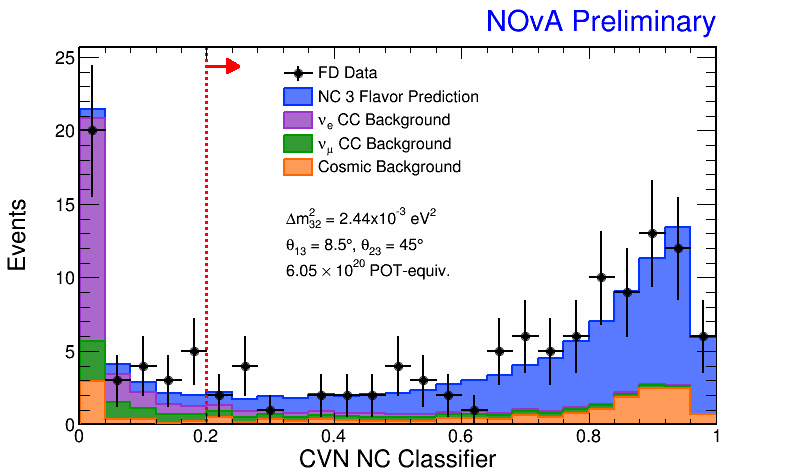
\includegraphics[width=.47\textwidth]{figures/FDDataMC/FDCVNStack.png}} \\
  \end{tabular}
  \caption[FD Data/MC Comparison: CVN Distribution]{FD data/MC comparison of the CVN distribution. The dashed line and arrow indicate the region kept for the analysis.}
  \label{fig:FDDataMCNCSel}
\end{figure}

\begin{figure}[htbp]
  \centering
  \begin{tabular}{c c}
    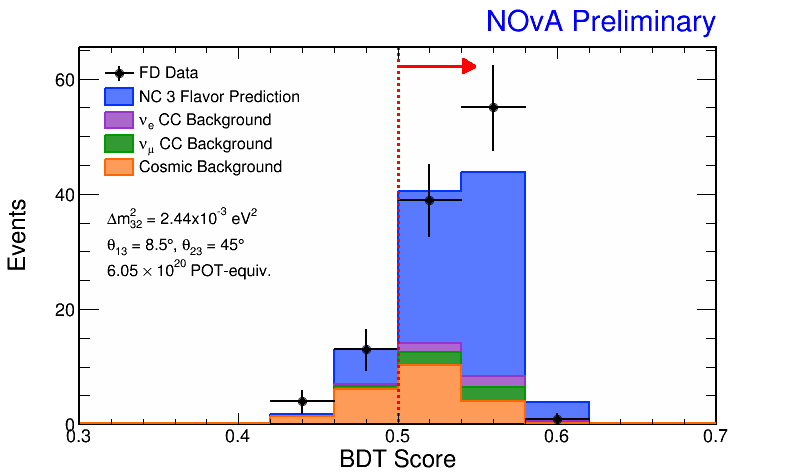
\includegraphics[width=.47\textwidth]{figures/FDDataMC/FDCosBDTStack.png} &
    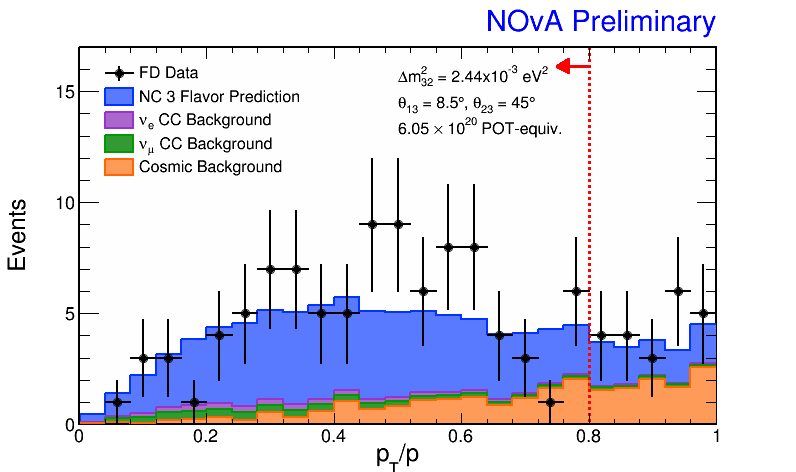
\includegraphics[width=.47\textwidth]{figures/FDDataMC/FDPTPStack.png} \\
    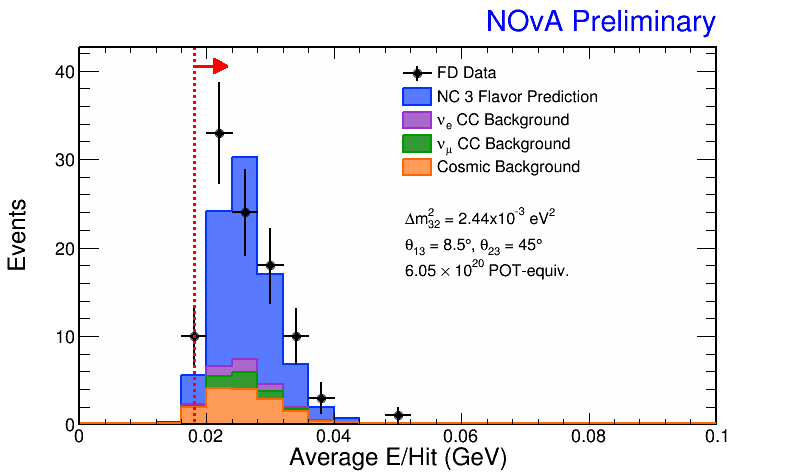
\includegraphics[width=.47\textwidth]{figures/FDDataMC/FDEperHitStack.png} &
    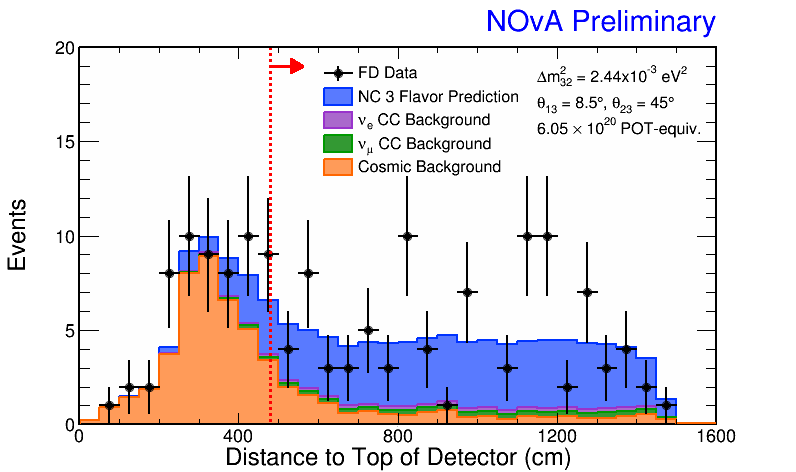
\includegraphics[width=.47\textwidth]{figures/FDDataMC/FDDistTopStack.png} \\
  \end{tabular}
  \caption[FD Data/MC Comparison: Cosmic Rejection Variable Distributions]{FD data/MC comparisons of the variables used for cosmic rejection. The dashed lines and arrows indicate the regions kept for the analysis.}
  \label{fig:FDDataMCCosRej}
\end{figure}